% !TeX root = ../main.tex
% Add the above to each chapter to make compiling the PDF easier in some editors.

\section{Design}
\subsection{User Interface}
\subsection{Page Structure and Navigation}
\subsubsection{}

\section{Data Structure}
\subsection{Overall Project Structure}
\subsection{Input File and Benchmark Data}


\subsubsection{Import of Performance Data}

The first step, working with the Benchy Viewer is to import a file containing the performance data which should be visualised. The file needs to follow the format introduced in Section \ref{sec:input-file-structure}. Figure~\ref{fig:input-process-flow} summarizes the import of the input file in a process diagram.

\begin{figure}[h]
  \centering
  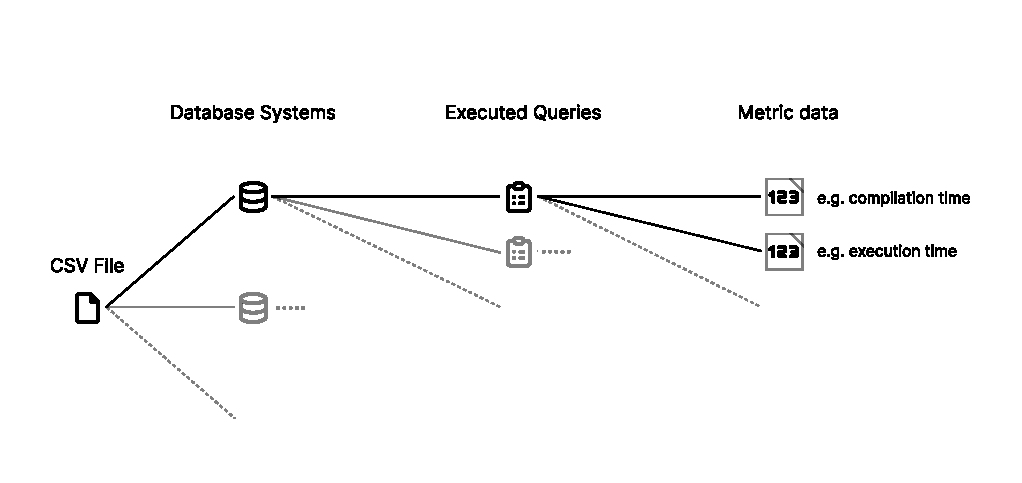
\includegraphics[width=1\linewidth]{figures/csv-structure.pdf}
  \caption{Import process of input data}
  \label{fig:input-process-flow}
\end{figure}

Chart beschreiben.


\subsection{Plot Options}
\subsection{Visualisation Arrangement Data Structure}
\subsection{Query Plan}
\subsubsection{Visualisation Parameters}
\subsubsection{Query Plan Data Structure}

\section{Integration of Plotly-React for Data Visualisation}
\subsection{Types of Plots and Charts}
\subsection{Hover Feature}
\subsection{Selected Query Feature}

\section{Integration of semantic-diff-tool}\label{sec:semantic-diff-integration}
\subsection{Business Logic}
\subsection{Settings}
\subsection{UI}